\documentclass[a4paper]{article}

%====================== PACKAGES ======================

\usepackage[french]{babel}
\usepackage[utf8x]{inputenc}
%pour gérer les positionnement d'images
\usepackage{float}
\usepackage{amsmath}
\usepackage{graphicx}
\usepackage[colorinlistoftodos]{todonotes}
\usepackage{url}
%pour les informations sur un document compilé en PDF et les liens externes / internes
\usepackage{hyperref}
%pour la mise en page des tableaux
\usepackage{array}
\usepackage{tabularx}
%pour utiliser \floatbarrier
%\usepackage{placeins}
%\usepackage{floatrow}
%espacement entre les lignes
\usepackage{setspace}
%modifier la mise en page de l'abstract
\usepackage{abstract}
%police et mise en page (marges) du document
\usepackage[T1]{fontenc}
\usepackage[top=2cm, bottom=2cm, left=2cm, right=2cm]{geometry}
%Pour les galerie d'images
\usepackage{subfig}
%landscape
\usepackage{pdflscape}

%====================== INFORMATION ET REGLES ======================

%rajouter les numérotation pour les \paragraphe et \subparagraphe
% \setcounter{secnumdepth}{4}
% \setcounter{tocdepth}{4}

\hypersetup{							% Information sur le document
pdfauthor = {Guillaume Clochard
			Thomas Coquereau},			% Auteurs
pdftitle = {Mini-Projet d'Intelligence Artificiel
			Emploi du temps à Polytech Nantes},			% Titre du document
pdfsubject = {Compte Rendu Mini-Projet},		% Sujet
pdfkeywords = {},	% Mots-clefs
pdfstartview={FitH}}					% ajuste la page à la largueur de l'écran
%pdfcreator = {MikTeX},% Logiciel qui a crée le document
%pdfproducer = {}} % Société avec produit le logiciel

%======================== DEBUT DU DOCUMENT ========================

\begin{document}

% %régler l'espacement entre les lignes
% \newcommand{\HRule}{\rule{\linewidth}{0.5mm}}
% %espacement entre les lignes d'un tableau
% \renewcommand{\arraystretch}{1.5}

\title{Mini-Projet d'Intelligence Artificiel \\
    Emploi du temps à Polytech Nantes}
\author{Guillaume Clochard, Thomas Coquereau}
\maketitle

% \tableofcontents

% \thispagestyle{empty}
% \setcounter{page}{0}
%ne pas numéroter le sommaire

%====================== INCLUSION DES PARTIES ======================

\section{Introduction}

Ce rapport présente un premier travail effectué dans le cadre du Mini-Projet
d'Intelligence Artificielle.
Il consiste en la planification de l'emploi du temps à Polytech Nantes.
Ce premier rendu s'attarde sur la modélisation générale du problème ainsi qu'une
première proposition de solution.


\newpage

\section{UML}
\begin{center}
	\begin{figure}[t]
	   \caption{\label{1} Diagramme de classe}
	   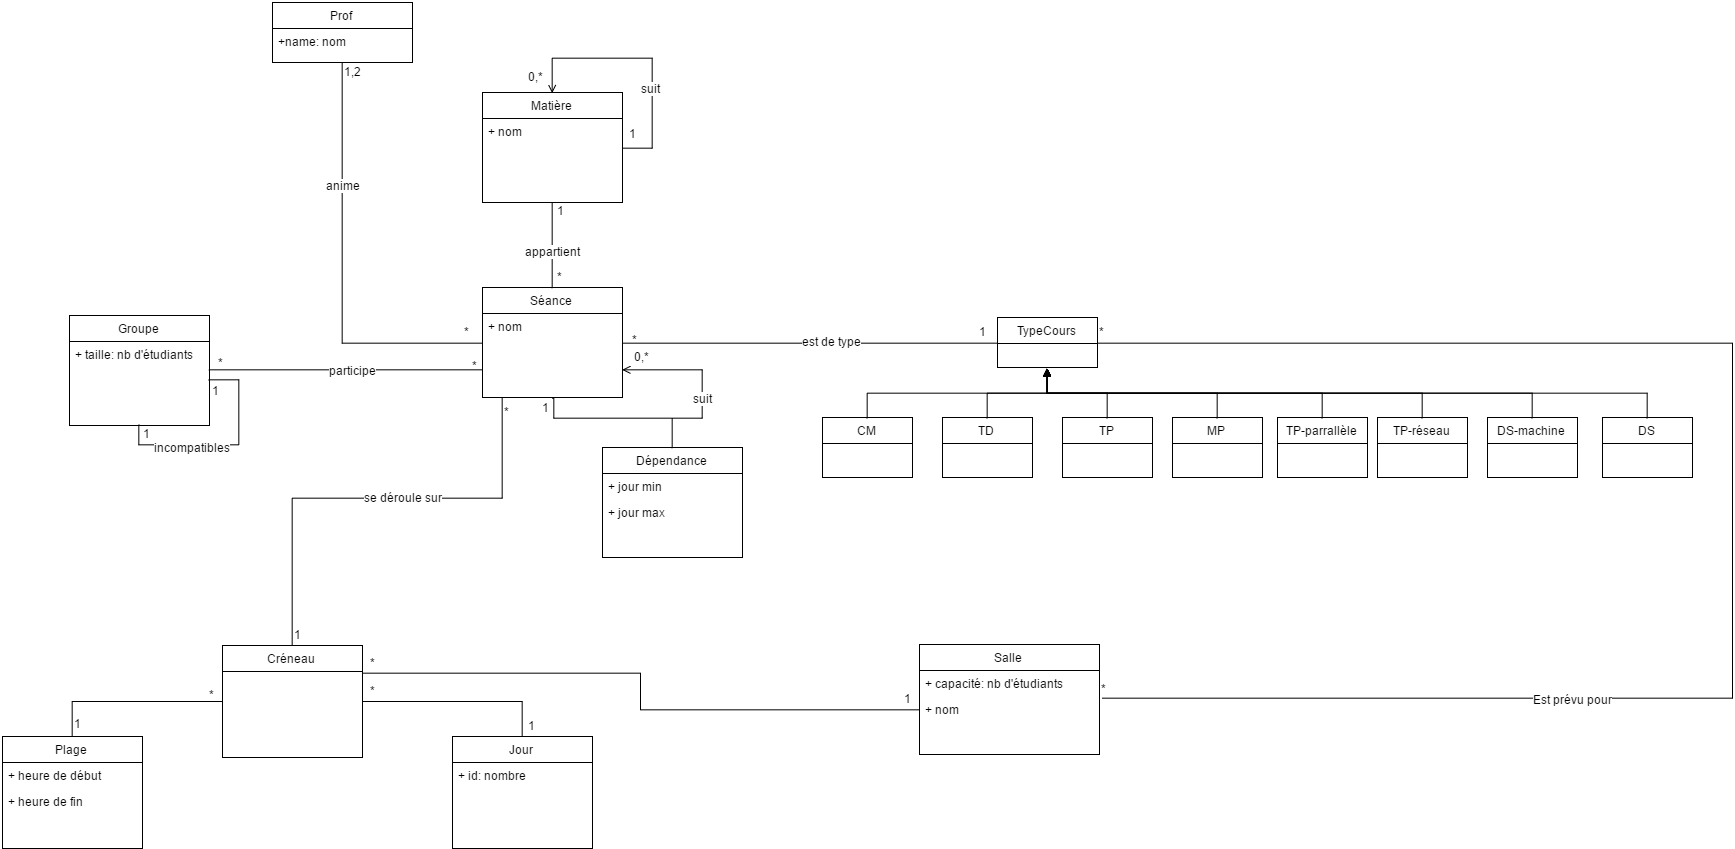
\includegraphics[keepaspectratio=true,width=17cm]{diagrammeClasse.png}
	\end{figure}
\end{center}
Voici le diagramme de classe décrivant les données nécessaires à la gestion de l'emploi du temps.
Comme on peut le constater, on regroupe l'ensemble des données nécessaires et déterminées à l'avance dans des Séances. A savoir : le(s) groupe(s) d'étudiants concerné(s), le professeur, la matière, ainsi que le type de cours. Ensuite ces séances vont être associées à des créneaux par notre solution. Les créneaux étant le regroupement d'un jour, une plage horaire et une salle.
Un peu noter des détails intéressants, sur Groupe, il y a la notion d'incompatibilité qui permet de définir lorsqu'il est possible pour deux groupes d'avoir cours sur une même plage horaire. Sur matière on à la notion de suite, lorsqu'une matière débute après la fin d'une autre (cf Mini-Projet d'IA qui suit le cours d'IA). Et enfin sur séance, on a la notion de suite aussi qui décrit une nombre de jours minimum et maximum avant le prochain cours de la même matière.

\end{document}
